\chapter{State-of-the-Art} \label{chap:sota}

\section*{}

\section{Introduction}

- explain gene expression

- explain importance and applications of gene expression profilling

- explain that nowadays sequencing data is easier and cheaper to obtain, but
  harder to process

- explain that there are several techniques to obtain gene expression
  information

- explain that in the thesis only RNA-Seq will be analysed

\begin{figure}[!htb]
  \begin{center}
    \leavevmode
    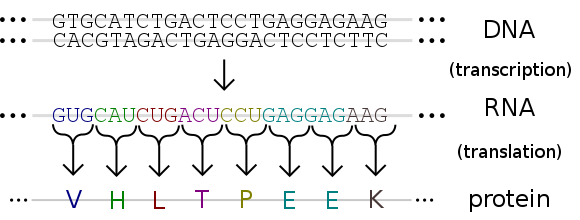
\includegraphics[width=0.6\textwidth]{gene_expr}
    \caption{Representation of the gene expression process\protect\footnotemark}
    \label{fig:arch}
  \end{center}
\end{figure}
\footnotetext{Image taken from \url{http://en.wikipedia.org/wiki/File:Genetic\_code.svg}.}

\section{Genome Assembly and \rnaseq}\label{sec:assembly}

\subsection{\rnaseq{} Tools}\label{sec:seqtools}

\subsection{Relevant Standard File Formats}\label{sec:formats}

\section{Data Mining}\label{sec:mlearning}

\subsection{Data Analysis Algorithms}\label{sec:minalgo}

\subsection{Data Analysis Tools}\label{sec:mintools}

\section{Chapter Conclusions}
